% !TEX encoding = UTF-8 Unicode
%%%%%%%%%%%%%%%%%%%%%%%%%%%%%%%%%%%%%%%%%
% Beamer Presentation
% LaTeX Template
% Version 1.0 (10/11/12)
%
% This template has been downloaded from:
% http://www.LaTeXTemplates.com
%
% License:
% CC BY-NC-SA 3.0 (http://creativecommons.org/licenses/by-nc-sa/3.0/)
%
%%%%%%%%%%%%%%%%%%%%%%%%%%%%%%%%%%%%%%%%%

%----------------------------------------------------------------------------------------
%	PACKAGES AND THEMES
%----------------------------------------------------------------------------------------

\documentclass{beamer}

\mode<presentation> {

% The Beamer class comes with a number of default slide themes
% which change the colors and layouts of slides. Below this is a list
% of all the themes, uncomment each in turn to see what they look like.

%\usetheme{default}
%\usetheme{AnnArbor}
%\usetheme{Antibes}
%\usetheme{Bergen}
%\usetheme{Berkeley}
%\usetheme{Berlin}
%\usetheme{Boadilla}
%\usetheme{CambridgeUS}
%\usetheme{Copenhagen}
%\usetheme{Darmstadt}
%\usetheme{Dresden}
%\usetheme{Frankfurt}
%\usetheme{Goettingen}
%\usetheme{Hannover}
%\usetheme{Ilmenau}
%\usetheme{JuanLesPins}
%\usetheme{Luebeck}
\usetheme{Madrid}
%\usetheme{Malmoe}
%\usetheme{Marburg}
%\usetheme{Montpellier}
%\usetheme{PaloAlto}
%\usetheme{Pittsburgh}
%\usetheme{Rochester}
%\usetheme{Singapore}
%\usetheme{Szeged}
%\usetheme{Warsaw}

% As well as themes, the Beamer class has a number of color themes
% for any slide theme. Uncomment each of these in turn to see how it
% changes the colors of your current slide theme.

%\usecolortheme{albatross}
%\usecolortheme{beaver}
%\usecolortheme{beetle}
%\usecolortheme{crane}
%\usecolortheme{dolphin}
%\usecolortheme{dove}
%\usecolortheme{fly}
%\usecolortheme{lily}
%\usecolortheme{orchid}
%\usecolortheme{rose}
%\usecolortheme{seagull}
%\usecolortheme{seahorse}
%\usecolortheme{whale}
%\usecolortheme{wolverine}

%\setbeamertemplate{footline} % To remove the footer line in all slides uncomment this line
%\setbeamertemplate{footline}[page number] % To replace the footer line in all slides with a simple slide count uncomment this line

%\setbeamertemplate{navigation symbols}{} % To remove the navigation symbols from the bottom of all slides uncomment this line
}

\usepackage{graphicx} % Allows including images
\usepackage{booktabs} % Allows the use of \toprule, \midrule and \bottomrule in tables
\usepackage{xeCJK}
\usepackage{color}
\usepackage{listings}
\usepackage{tikz}


%----------------------------------------------------------------------------------------
%	TITLE PAGE
%----------------------------------------------------------------------------------------

\title[database]{数据库技术} % The short title appears at the bottom of every slide, the full title is only on the title page

\author{张海宁} % Your name
\institute[贵大计算机] % Your institution as it will appear on the bottom of every slide, may be shorthand to save space
{
贵州大学 \\ % Your institution for the title page
\medskip
\textit{hnzhang1@gzu.edu.cn} % Your email address
}
\date{\today} % Date, can be changed to a custom date

\begin{document}

\begin{frame}
\titlepage % Print the title page as the first slide
\end{frame}

\begin{frame}
\frametitle{Overview} % Table of contents slide, comment this block out to remove it
\tableofcontents % Throughout your presentation, if you choose to use \section{} and \subsection{} commands, these will automatically be printed on this slide as an overview of your presentation
\end{frame}

%----------------------------------------------------------------------------------------
%	PRESENTATION SLIDES
%----------------------------------------------------------------------------------------

%------------------------------------------------
\section{MySQL} % Sections can be created in order to organize your presentation into discrete blocks, all sections and subsections are automatically printed in the table of contents as an overview of the talk
%------------------------------------------------
\begin{frame}
\frametitle{MySQL}
Many of the world's largest and fastest-growing organizations including Facebook, Google, Adobe, Alcatel Lucent and Zappos rely on MySQL to save time and money powering their high-volume Web sites, business-critical systems and packaged software.
\end{frame}
%\subsection{System Calls} % A subsection can be created just before a set of slides with a common theme to further break down your presentation into chunks

\begin{frame}
\frametitle{database popularity}
\textbf{Most popular databases in 2017 according to StackOverflow survey}
\begin{figure}
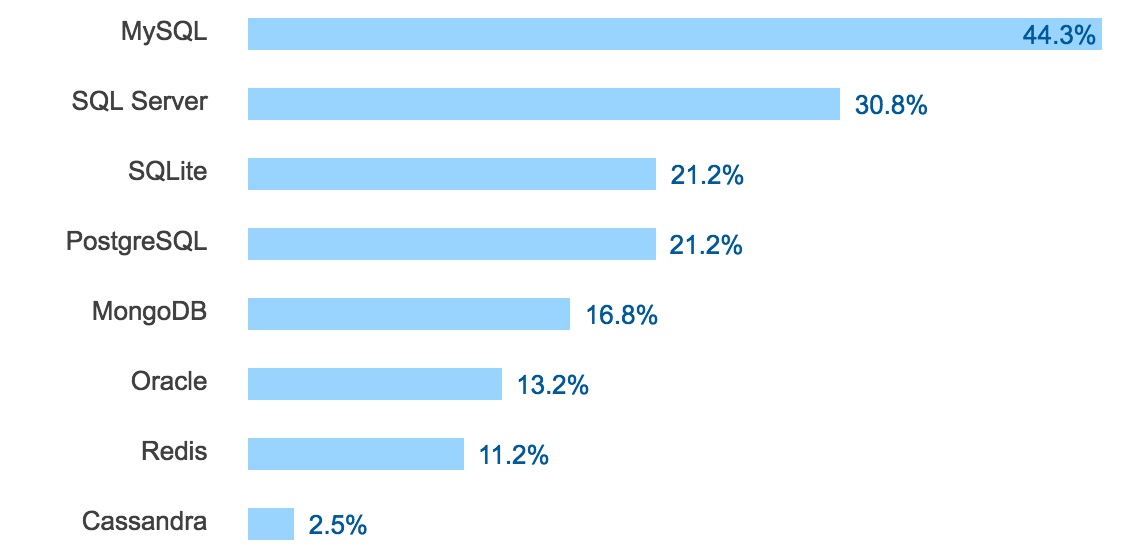
\includegraphics[width=1\linewidth]{sql1.png}
\end{figure}
\url{https://www.eversql.com/most-popular-databases-in-2017-according-to-stackoverflow-survey/}
\end{frame}
\begin{frame}
\frametitle{分析}
\begin{enumerate}
\item
The most popular database is MySQL, and not by far comes SQL Server. Almost half of the developers who answered the survey (44.3\% out of 36,935 responders) are using MySQL. It seems RDBMS databases and specifically MySQL are not going anywhere anytime soon.

\item
RDBMS databases are still significantly more common than NoSQL databases such as MongoDB.
\item
Relatively new technologies are starting to gain market share in the databases world – Redis (first release at 2009) and Cassandra (first release at 2008).
\item
Almost 1/4 of all programmers (23.3\%) are using SQLite, which is a lite SQL database which is based on a single file. This small database software is gaining popularity among developers, probably mostly for simple and standalone applications.

\end{enumerate}
\end{frame}
\begin{frame}
\frametitle{download and install MySQL}
\begin{block}{Download MySQL and MySQL connectors}
\url{https://dev.mysql.com/downloads/workbench/}\textcolor{red}{(GUI工具)}
\url{https://dev.mysql.com/downloads/mysql/}
\url{https://dev.mysql.com/downloads/connector/j/}
\end{block}
\begin{block}{Install}
一般地,对于MySQL和MySQL workbench默认下一步安装即可。
MySQL Connector/J 解压,将mysql-connector-java-xxx-bin.jar文件加入到eclipse中项目的库文件路径中。(在eclipse中,右键项目->属性->库->添加外部jar文件)
\end{block}
\end{frame}
%----------------------------------------
\section{JDBC}
\begin{frame}
\frametitle{JDBC}
Java Database Connectivity (JDBC) is an application programming interface (API) for the programming language Java, which defines how a client may access a database. 

JDBC是oracle公司提出的一个标准,其具体实现由各家数据库公司自己进行。
\end{frame}
\begin{frame}
\frametitle{JDBC的功能}
\begin{enumerate}
\item
同数据库建立连接
\item
向数据库发送sql语句
\item
处理从数据库返回的结果
\end{enumerate}
\end{frame}
\begin{frame}

\frametitle{JDBC中常用的接口}
\begin{table}
\begin{tabular}{l l l l }
\toprule
\textbf{接口} & \textbf{作用}\\
\midrule
Driver & 负责加载驱动 \\
DriverManager & 负责管理驱动和连接数据库\\
Connection & 管理某个数据库连接 \\
Statement  & 执行sql语句,并返回结果 \\
ResultSet & 获得检索结果 \\
\bottomrule
\end{tabular}
\caption{JDBC的常用接口}
\end{table}
\end{frame}
%--------------------------------------
\section{连接数据库}
\begin{frame}
\frametitle{连接数据库的一般流程}
jsp连接数据库的一般流程如下:
\begin{enumerate}
\item
加载jdbc驱动程序
\item
创建数据库连接
\item
执行sql语句
\item
获取查询结果
\item
关闭连接
\end{enumerate}
\end{frame}
\begin{frame}[fragile]
\frametitle{加载jdbc驱动}
\begin{lstlisting}
<%@ page language="java" pageEncoding="UTF-8"%>
<%@ page import="java.sql.*" %>
<%
  try{
  
    Class.forName("com.mysql.jdbc.Driver");
    
  }catch(ClassNotFoundException e){
    System.out.println("驱动加载失败!");
    e.printStackTrace();
  }
%>
\end{lstlisting}
\end{frame}

\begin{frame}[fragile]
\frametitle{建立数据库连接}
使用\textcolor{red}{DriverManager}类的getConnection()方法建立sql连接。
\begin{lstlisting}
<%
  try{
    Class.forName("com.mysql.jdbc.Driver");
    
    Connection conn = DriverManager.getConnection(
        "jdbc:mysql://localhost","root","password");
  
  }catch(Exception e){
    System.out.println("出现错误,具体内容如下:");
    e.printStackTrace();
  }
%>
\end{lstlisting}
\end{frame}


\begin{frame}[fragile]
\frametitle{执行sql语句}
使用Connection类的对象\textcolor{red}{conn的createStatement()方法}创建Statement类的对象\textcolor{red}{st},再使用st对象来执行sql语句(executeQuery()或executeUpdate())。
\begin{lstlisting}
<%
  try{
    Class.forName("com.mysql.jdbc.Driver");
    Connection conn = DriverManager.getConnection(
        "jdbc:mysql://localhost/","root","password");
    Statement st = conn.createStatement();
    st.executeQuery("show databases;");
}catch(Exception e){
    System.out.println("出现错误,具体内容如下:");
    e.printStackTrace();
}
%>
\end{lstlisting}
\end{frame}


\begin{frame}[fragile]
\frametitle{获取查询结果并关闭数据库连接}
通过Statement类的对象\textcolor{red}{st}来执行sql语句(executeQuery()或executeUpdate()),会返回一个ResultSet类的对象\textcolor{red}{rs},rs对象拥有一些方法可以获取查询到的值。
\begin{lstlisting}
<%
try{	
   Class.forName("com.mysql.jdbc.Driver");
   Connection conn = DriverManager.getConnection(
    "jdbc:mysql://localhost/","root","password");
   Statement st = conn.createStatement();
   ResultSet rs = st.executeQuery("show databases;");
   while(rs.next()){
   String str = rs.getString(1);
   System.out.println(str);
}
    conn.close();
}catch(Exception e){ e.printStackTrace(); }
%>
\end{lstlisting}
\end{frame}


\begin{frame}[fragile]
\frametitle{完整java代码}
\begin{lstlisting}
<%
try{
   Class.forName("com.mysql.jdbc.Driver");
   Connection conn = DriverManager.getConnection(
    "jdbc:mysql://localhost/","root","password");
   Statement st = conn.createStatement();
   ResultSet rs = st.executeQuery("show databases;");
   int column = rs.getMetaData().getColumnCount();
   System.out.println(column);
   while(rs.next()){
     System.out.println(rs.getString(1));
   }
    conn.close();
}catch(Exception e){ e.printStackTrace(); }
%>
\end{lstlisting}
\end{frame}
%---------------------------------------
\section{实例}
\begin{frame}
\frametitle{建表}
接下来本ppt参照以下ER图建立数据库及表以进行演示。
\begin{figure}
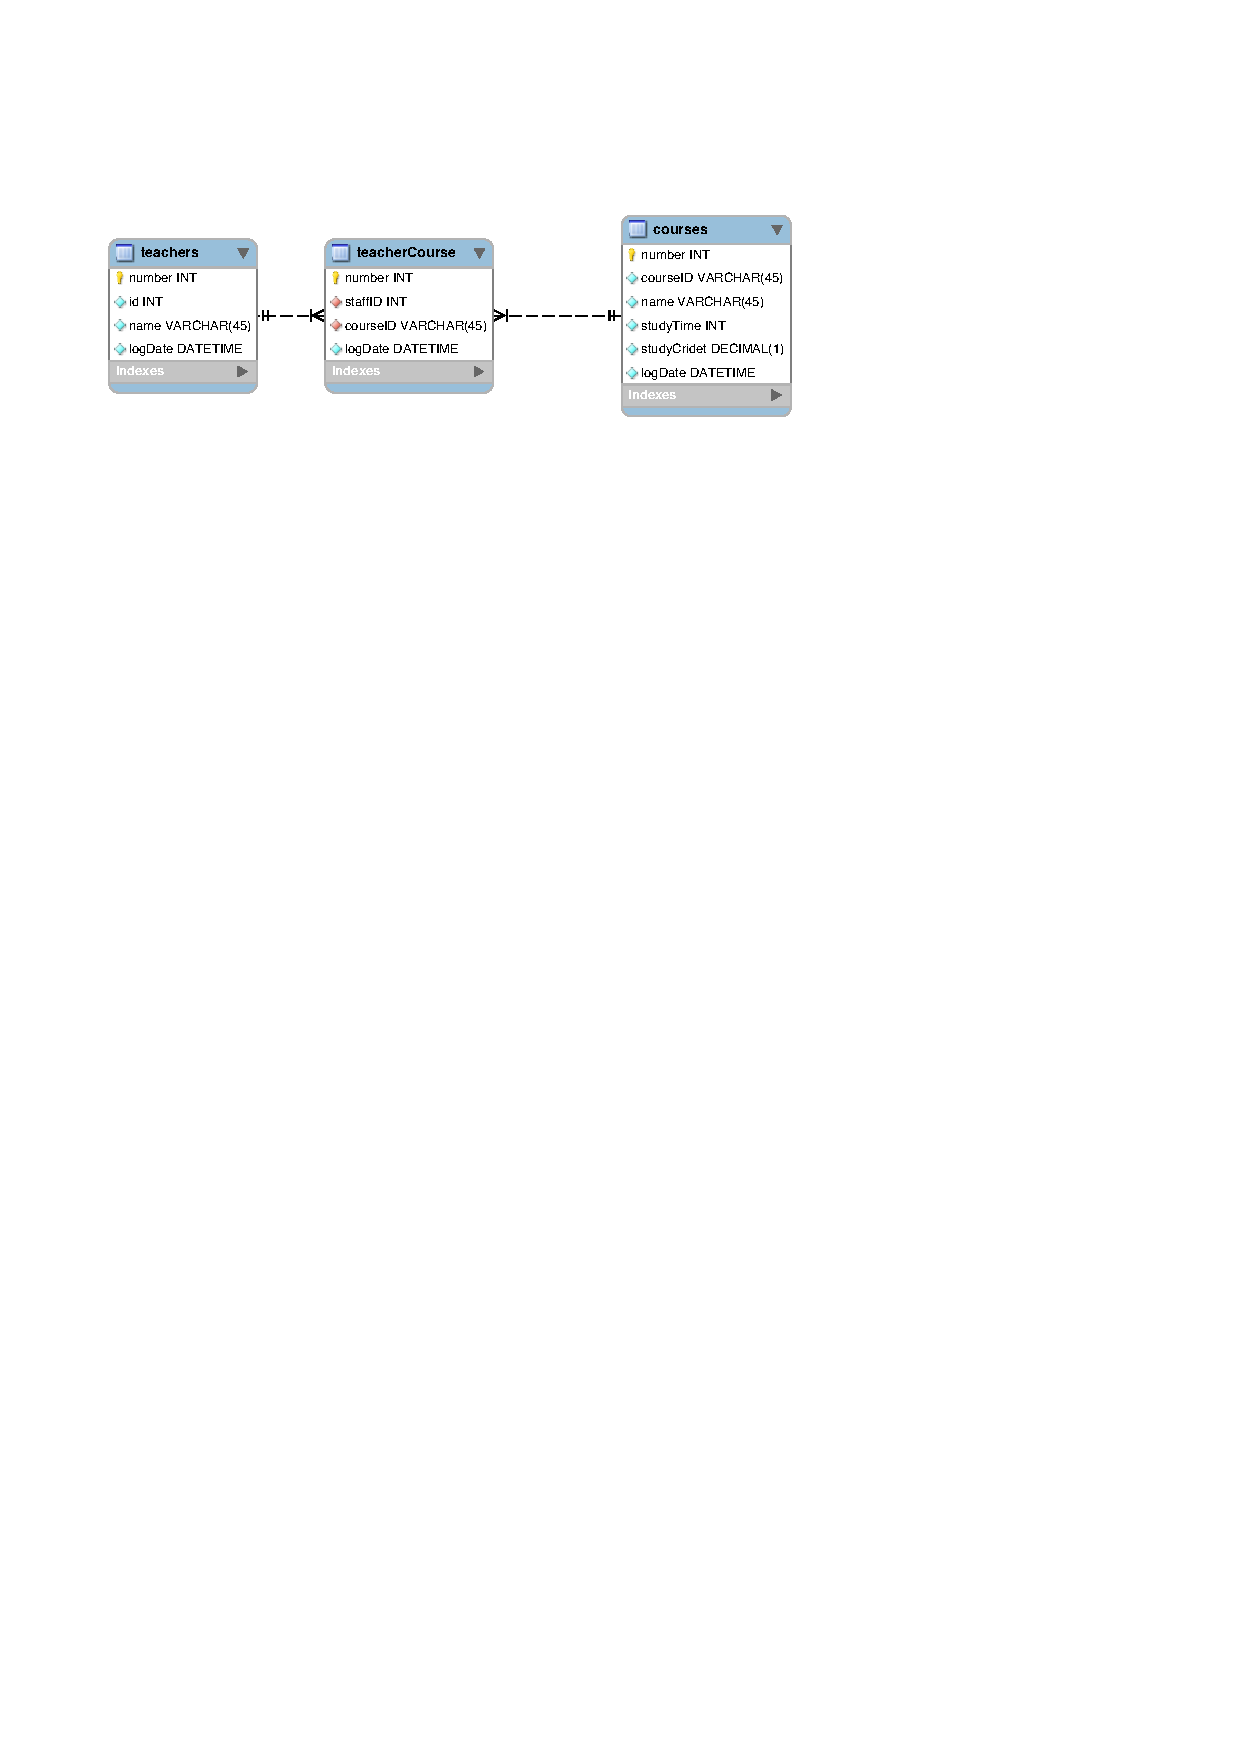
\includegraphics[height=27cm]{sql2.pdf}
\end{figure}
\end{frame}
\subsection{写数据到数据库}
\begin{frame}
\frametitle{信息录入页面}
\begin{figure}
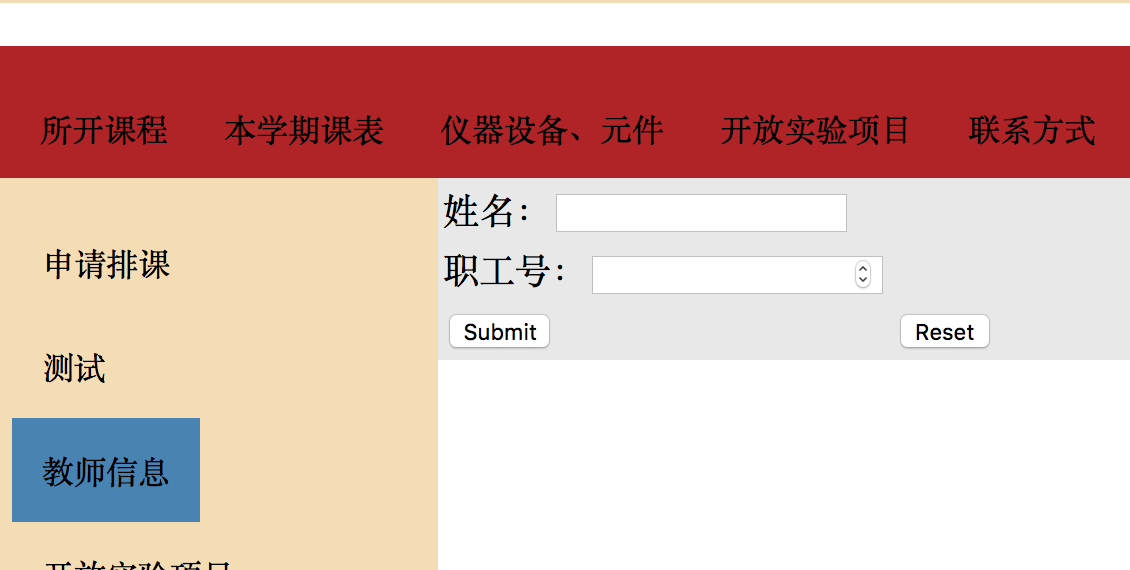
\includegraphics[width=1\linewidth]{sql3.png}
\end{figure}
\end{frame}
\begin{frame}[fragile]
\frametitle{信息录入界面关键代码}
\begin{lstlisting}
<form action="teacher_add.jsp" method="post">
<table>
<tr><td>姓名:<input type="text" name="nm"></td></tr>
<tr><td>
职工号:<input type="number" name="staffid" min=20060001 >
</td></tr>
<tr><td><input type="submit"></td>
<td><input type="reset"></td></tr>
</table>
</form>

\end{lstlisting}
\end{frame}

\begin{frame}[fragile]
\frametitle{写入数据库代码1/2}
\begin{lstlisting}
String teacher_name = 
    request.getParameter("nm");
int teacher_id = 
  Integer.parseInt(request.getParameter("staffid"));
Calendar c = Calendar.getInstance();
String d = c.get(Calendar.YEAR)+"-"+
    (c.get(Calendar.MONTH)+1)+"-"+
    c.get(Calendar.DATE)+" "+
    c.get(Calendar.HOUR_OF_DAY)+":"+
    c.get(Calendar.MINUTE)+":"+
    c.get(Calendar.SECOND);


\end{lstlisting}
\end{frame}

\begin{frame}[fragile]
\frametitle{写入数据库代码2/2}
\begin{lstlisting}
String sql = 
 "insert into teachers (id,name,logDate) values(?,?,?)";
int rz=0;
try{		
  Class.forName("com.mysql.jdbc.Driver");
  Connection conn = DriverManager.getConnection(
   "jdbc:mysql://localhost/lab","root","password");
  PreparedStatement prep = conn.prepareStatement(sql);
  prep.setInt(1, teacher_id);
  prep.setString(2,teacher_name);
  prep.setString(3, d);
  rz = prep.executeUpdate();
  System.out.println(rz);
  conn.close();
  if(rz==1){	
    response.sendRedirect("teacher.jsp");
  }
}catch(Exception e){ e.printStackTrace();}
\end{lstlisting}
\end{frame}
\subsection{查询数据}
\begin{frame}
\frametitle{查询数据结果}
\begin{figure}
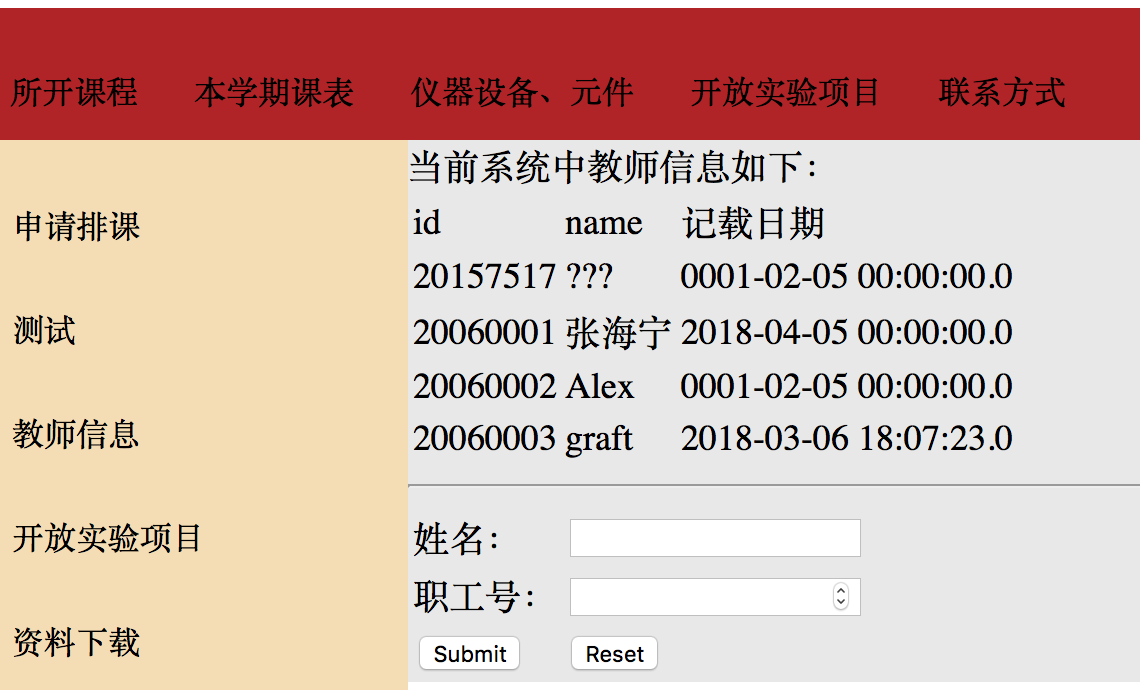
\includegraphics[width=1\linewidth]{sql4.png}
\end{figure}
\end{frame}

\begin{frame}[fragile]
\frametitle{查询数据关键代码}
\begin{lstlisting}
<table>
<tr><td>id</td><td>name</td><td>记载日期</td></tr>
<%	
 Class.forName("com.mysql.jdbc.Driver");
 Connection conn = DriverManager.getConnection(
  "jdbc:mysql://localhost/lab","root","password");
 Statement st = conn.createStatement();
 String sql = "select * from teachers;";
 ResultSet rs = st.executeQuery(sql);
 while(rs.next()){
 out.print("<tr><td>"); out.print(rs.getInt(2));
 out.print("</td><td>"); out.print(rs.getString(3));
 out.print("</td><td>"); out.print(rs.getString(4));
 out.print("</td></tr>");
%>
</table>
\end{lstlisting}
\end{frame}
%---------------------------------------
\section{session}
\begin{frame}
\frametitle{session}
与cookie对象类似,session对象也是用来保存与用户请求有关的一些数据。服务器为每个用户生成一个session对象,用于保存用户的信息,跟踪用户的操作状态。session使用Map这种数据结构来保存数据。
其常用方法如下表所示:

\begin{table}
\begin{tabular}{l l l}
\toprule
\textbf{方法}  & \textbf{说明}\\
\midrule
setAttribute(String name, Object obj) &   设置属性及对应的值\\
invalidate() &   销毁session对象\\
getAttribute(String name) &  获得指定属性的值\\
getAttributeNames() &  获得session对象中所有的属性的名字\\
\bottomrule
\end{tabular}
\caption{session对象常用方法}
\end{table}
\end{frame}
\subsection{session的使用}
\begin{frame}[fragile]
\frametitle{判断session中是否有需要的值}
\textbf{nav.jsp}
\begin{lstlisting}
<%	
String user="";
Enumeration<String> enu = session.getAttributeNames();
while(enu.hasMoreElements()){
String attr = enu.nextElement();
if(attr.equals("user")){
user = (String)session.getAttribute("user");
out.print("你好,"+user+"。");
out.print("<form action=\"logout.jsp\" method=\"post\">");
out.print("<input type=\"submit\" value=\"logout\"></form>");
 break; } }
if(user.equals("")){
out.print("<form action=\"login.jsp\" method=\"post\">");
out.print("ID:<input type=\"number\"  name=\"id\">");
out.print("<input type=\"submit\" value=\"login\"></form>"); }
%>
\end{lstlisting}
\end{frame}

\begin{frame}[fragile]
\frametitle{查询数据库,创建session}
\textbf{login.jsp}
\begin{lstlisting}
<%
int id = Integer.parseInt(request.getParameter("id"));
Db db = new Db();
Connection conn = db.getConnection();
String sql = "select name from teachers where id=?";
PreparedStatement pst = conn.prepareStatement(sql);
pst.setInt(1, id);
ResultSet rs = pst.executeQuery();
if(rs.first()){
  session.setAttribute("id", id);
  session.setAttribute("user", rs.getString("name"));
}
conn.close();
response.sendRedirect("index.jsp");
%>
\end{lstlisting}
\end{frame}
\begin{frame}
\frametitle{before and after login}
\begin{figure}
before login:
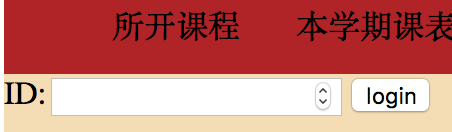
\includegraphics{sql5.png}

after login:
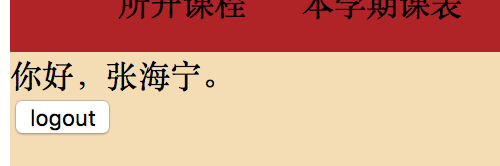
\includegraphics{sql6.png}
\end{figure}
\end{frame}

%------------------------------------------------
\begin{frame}
\frametitle{作业}

使用session对象,为本小组的项目增加登陆注销功能。
\end{frame}


%------------------------------------------------

\begin{frame}
\Huge{\centerline{The End}}
\end{frame}

%---------------------------------------
\begin{frame}
\frametitle{目录}
\begin{tikzpicture}
\node(/) at (7,10) {/};
\node(bin) at (5,8) {bin};
\node(home) at (7,8) {home};
\node(dev) at (9,8) {dev};
\draw (bin) -- (/) -- (dev);
\draw (/) -- (home);
\node (zhn) at (5,6) {zhn};
\node (wys) at (7,6) {wys};
\node (students) at (9,6) {students};
\draw (home) -- (zhn);  
\draw (home) -- (wys); 
\draw (home) -- (students); 
%\node (public\_html) at (3,4) {public\_html};
\node (linux) at (2,4) {linux};
\node (javaweb) at (7,4) {javaweb};
%\draw (zhn) -- (public\_html);
\draw (zhn) -- (linux);
\draw (zhn) -- (javaweb);


\end{tikzpicture}
\end{frame}


%----------------------------------------------------------------------------------------

\end{document} 